\section{Experimento 3} 

Este experimento trata sobre la medición de la inductancia de una bobina con un metodo alternativo, este metodo se basa en el principio de resonancia.

Este método consiste en conectar la misma con un condensador de valor conocido de
manera de formar un circuito resonante serie, y excitar el conjunto con una señal senoidal
de frecuencia variable, la cual deberá ajustarse hasta llegar a la condición de resonancia. 

\begin{figure}[H]
    \centering
    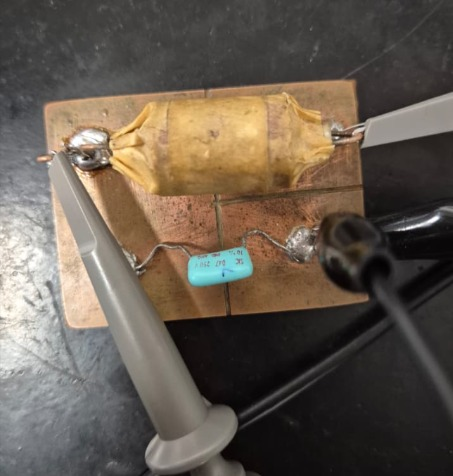
\includegraphics[width=0.5\textwidth]{images/circuitoaplicado3.jpeg}
    \caption{Circuito aplicado para la medición de la inductancia}
    \label{fig:conexiones5}
\end{figure}

Luego de conectar el circuito, se ajusta la frecuencia de la señal senoidal hasta alcanzar la frecuencia de resonancia $f_{0}$ observando que se produzca un máximo en $e_{c}$ (que debe coincidir con un mínimo en $e_{Tot}$) 

Consideramos una Voltaje de entrada de 4Vpp, y se observa que la señal de resonancia es la siguiente:

\begin{figure}[H]
    \centering
    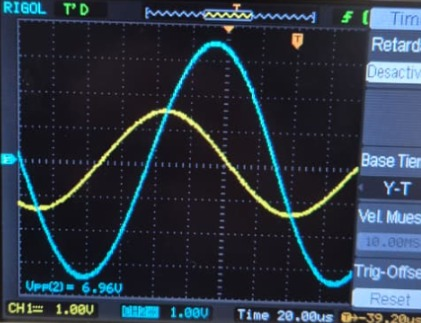
\includegraphics[width=0.5\textwidth]{images/señalresonancia.jpeg}
    \caption{Señal de resonancia}
    \label{fig:señalresonancia}
\end{figure}

En estas circunstancias se tomará el valor de
la frecuencia y se calculará la inductancia de la bobina mediante la fórmula de Thompson:

\begin{equation*}
   f_{0} = \frac{1}{2\pi \sqrt{LC}} 
\end{equation*}

\begin{equation*}
    L = \frac{1}{(2\pi f_{0})^{2}C} \rightarrow L = \frac{1}{(2\pi 6,7kHz)^{2} 47nF} = 12mH
\end{equation*}


Con este procedimiento también es posible determinar el factor de mérito (Q) de la
bobina. Esto es así dado que en un circuito resonante LC, el elemento que normalmente
tiene más pérdidas es la bobina, por lo que es posible asumir que el Q del circuito
resonante es directamente igual al Q de la bobina.

Sabiendo cuanto es el valor de nuestro $e_{c}$  podemos determinar los valores de la siguiente tabla:

\begin{table}[H]
\resizebox{\columnwidth}{!}{%
\begin{tabular}{|l|c|c|c|c|}
\hline
\multicolumn{1}{|c|}{\textbf{Condición}} & \textbf{f} & \textbf{$\mathbf{e_C}$ (C1)} & \textbf{$\mathbf{e_{total}}$ (C2)} & \textbf{$Q=\mathbf{e_C}/\mathbf{e_{total}}$} \\ \hline
$f_1(0.707* \mathbf{e_C} \text{ máximo})$ & 2,98kHz & 4,92Vpp & 3,4Vpp & ------------------ \\ \hline
$f_0(\mathbf{e_C} \text{ máximo})$ &6,7kHz & 6,96Vpp & 3Vpp & 2,32 \\ \hline
$f_2(0.707* \mathbf{e_C} \text{ máximo})$ & 8,98kHz & 4,92Vpp & 3,08Vpp & ------------------ \\ \hline
\end{tabular}%
}
\end{table}


\textbf{Cálculo y comparación del ancho de banda:}\\
A partir de las mediciones obtenidas, se determina el ancho de banda empírico ($B$):
\begin{equation*}
    B = f_2 - f_1 = 8,98 \text{ kHz} - 2,98 \text{ kHz} = 6 \text{ kHz}
\end{equation*}

Por otro lado, la aproximación teórica relaciona la frecuencia de resonancia y el factor de mérito:
\begin{equation*}
    B_{\text{teórico}} \approx \frac{f_0}{Q} = \frac{6,7 \text{ kHz}}{2,32} = 2,88 \text{ kHz}
\end{equation*}

\vspace{0.5cm}
\noindent
\textbf{Conclusión sobre el Experimento 3:}

Al comparar el ancho de banda medido ($6 \text{ kHz}$) con el teórico ($2,88 \text{ kHz}$), se observa una diferencia significativa. Se establece que la relación $f_0 / Q \approx B$ adquiere mayor exactitud cuanto menor sea el ancho de banda relativo $B/f_0$. En nuestra experiencia, el factor de mérito calculado resultó ser sumamente bajo ($Q = 2,32$), lo cual es indicativo de un circuito resonante con elevadas pérdidas resistivas. 



